\documentclass{article}
\usepackage{tabularx}
\usepackage{longtable}
\usepackage{array}
\usepackage{float}
\usepackage{listings}
\usepackage{amsmath}
\usepackage{amssymb}
\usepackage{mathtools}
\usepackage{amsfonts}
\usepackage{graphicx}
\usepackage[table]{xcolor}
\setlength{\arrayrulewidth}{0.5mm}
\graphicspath{ {./images/} }
\usepackage[margin=20mm]{geometry}
\renewcommand{\labelenumii}{\theenumii}
\renewcommand{\theenumii}{\theenumi.\arabic{enumii}.}
\renewcommand{\arraystretch}{1.5}
\newcommand{\f}[2]{f_{#1}(#2)}
\newcommand{\code}[1]{\texttt{#1}}
\DeclarePairedDelimiter{\ceil}{\lceil}{\rceil}
\DeclarePairedDelimiter{\set}{\left\{}{\right\}}
\DeclarePairedDelimiter{\parens}{\lparen}{\rparen}
\title{HW2 Report}
\date{}
\begin{document}
\maketitle
\section*{Part 1}
\subsection*{Q1:}
    \begin{figure}[H]
        \centering
        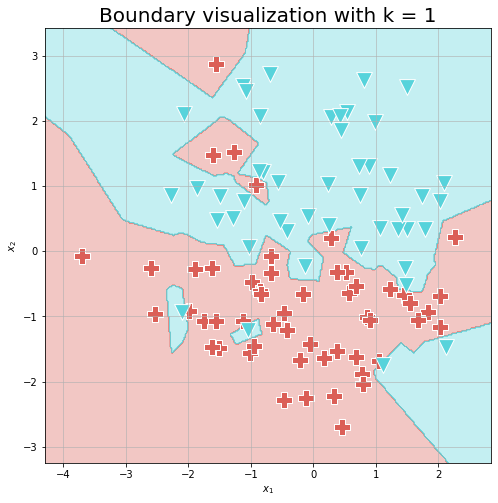
\includegraphics[scale=0.4]{q1_k1.png}
        \caption{Boundary Visualization for KNN with K = 1}
        \label{fig:q1_k1}
    \end{figure}
    \begin{figure}[H]
        \centering
        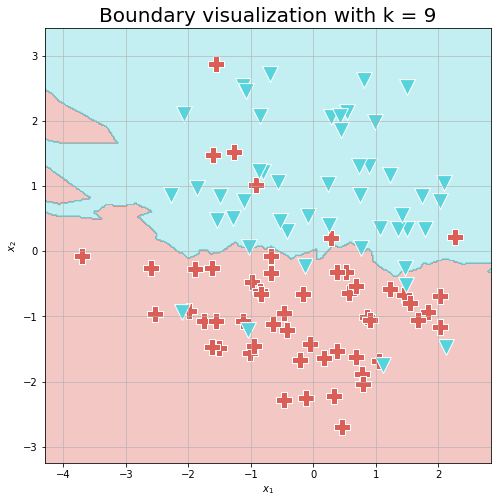
\includegraphics[scale=0.4]{q1_k9.png}
        \caption{Boundary Visualization for KNN with K = 9}
        \label{fig:q1_k9}
    \end{figure}
    \paragraph*{}
    As can be seen in figure \ref{fig:q1_k1}, the model with k equal to 1 caused overfitting to occur, as for every new sample point, its prediction took into account only the closest point to it, thereby increasing the complexity of the model since every new point is predicted locally. On the other hand, as can be seen in figure \ref{fig:q1_k9}, the model with k equal to nine takes into account the nine closest points to the sample being predicted, and therefore takes a broader outlook on the training data in-order to tdo the prediction, thereby lowering the complexity. But at the same time, we can see that a number of points were not classified correctly, and therefore this could indicate that this model is performing underfitting.
    
\subsection*{Q2:}
    \begin{figure}[H]
        \centering
        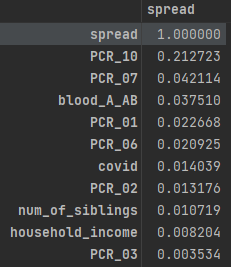
\includegraphics{images/q2.png}
        \caption{The 10 most correlated features to \code{spread}}
    \end{figure}
\subsection*{Q3:}
    \begin{figure}[H]
        \centering
        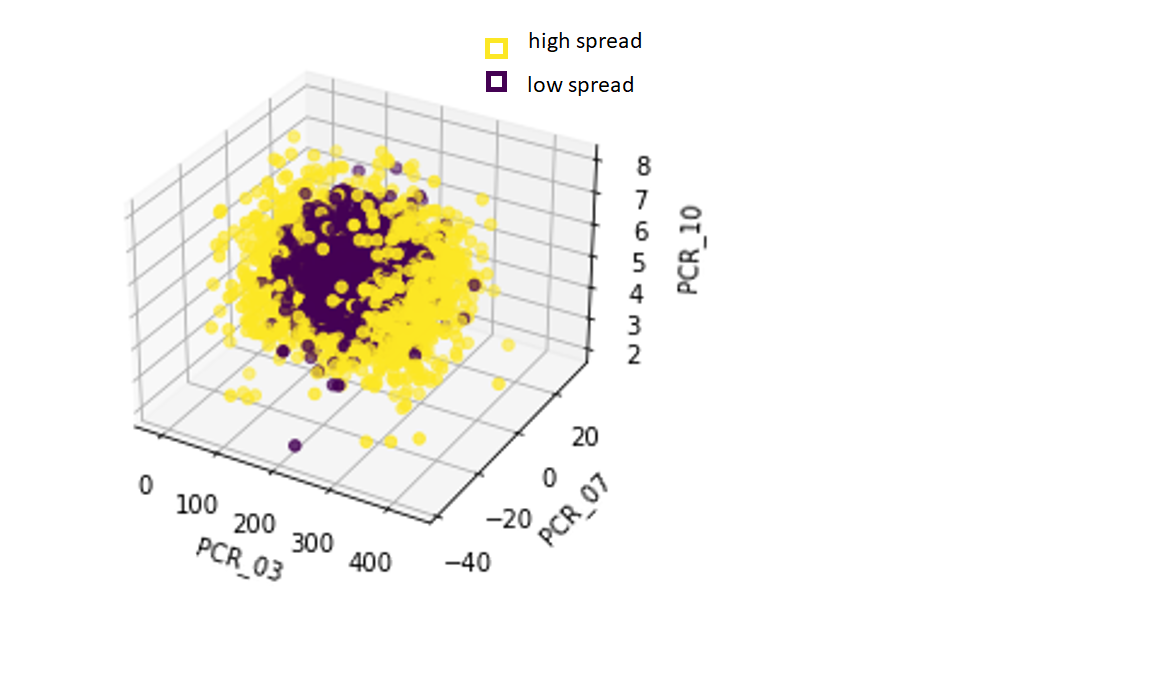
\includegraphics{images/q3.png}
        \caption{3D Scatter plot of \code{PCR\_03}, \code{PCR\_07}, and \code{PCR\_10} according to \code{spread}}
    \end{figure}
\subsection*{Q4:}
    \paragraph*{}
    The points with label -1 for \code{spread} are contained within an ellipsoid described by the following equation:
    \begin{align*}
        \frac{PCR\_03}{a^2} + \frac{PCR\_07}{b^2} + \frac{PCR\_10}{c^2} = 1
    \end{align*}
    where $a,b,c$ are positive real numbers.
\subsection*{Q5:}
    \paragraph*{}
    The training accuracy for $k=11$ is $81.333\%$.

\subsection*{Q6:}
    \paragraph*{}
    Z-score scaling scales the data of a feature by ensuring that they have zero mean and unit standard deviation, thereby causing the data to adhere to a normal distribution. Features scaled according to this technique have their outliers handled correctly, but no guarantee on the resulting range of the data is made, and the ranges of different features scaled according to Z-score may differ from each other. This technique is preferable in cases that have outliers and when the learning model assumes that the data adheres to a normal distribution . On-the-other-hand, the min-max technique involves scaling the data of a feature to a specific range (generally between 0 and 1). Contrary to the Z-score method, this technique guarantees a uniform range across features and maintains the original distribution of the data, but does not handle outliers well. Therefore, it would be preferable to use this technique only when the feature in question has no significant outliers and\_or the learning model to be used requires the feature data to fall within a certain range.
\subsection*{Q8:}
    \begin{figure}[H]
        \centering
        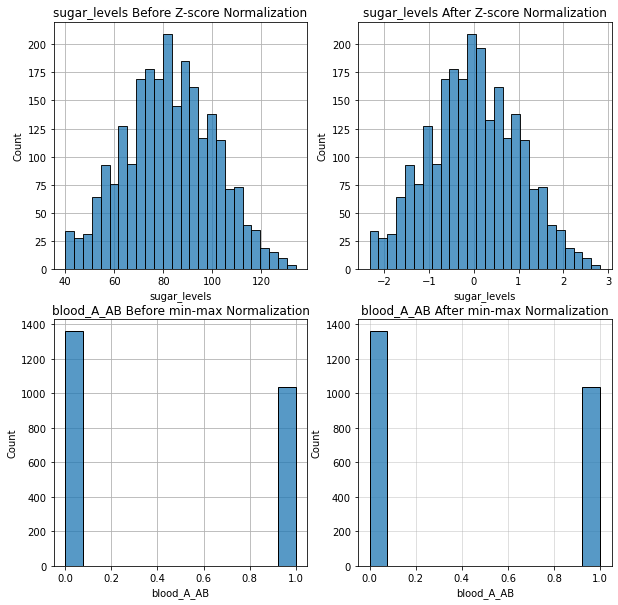
\includegraphics[scale=0.5]{q8_hists.png}
        \caption{Histogram Plots of \code{sugar\_levels} and \code{blood\_A\_AB} Before and After Normalization}
        \label{fig:q8_hist}
    \end{figure}
    \paragraph*{}
    We chose to do Z-score Normalization on \code{sugar\_levels} since it obeys an approximate normal distribution, as can be seen in figure \ref{fig:q8_hist}. On the other hand, we chose to do min-max normalization on \code{blood\_A\_AB}, since it does not obey a normal distribution.
\section*{Part 2}
\subsection*{Q11:}
    \begin{figure}[H]
        \centering
        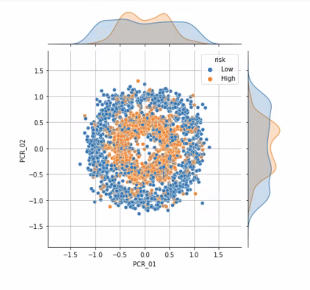
\includegraphics{q11_pcr_01_pcr_02_j_plot.png}
        \caption{Joint plot of PCR\_01 and PCR\_02 according to risk}
        \label{fig:pcr_01_pcr_02_j_plot}
    \end{figure}
    \paragraph*{}
    As can be seen from the scatter portion of the jointplot in figure \ref{fig:pcr_01_pcr_02_j_plot}, the plot is mostly separable into radiuses, and therefore it seems likely that \code{PCR\_01} and \code{PCR\_02} will be important in predicting the \code{risk} class.
    \begin{figure}[H]
        \centering
        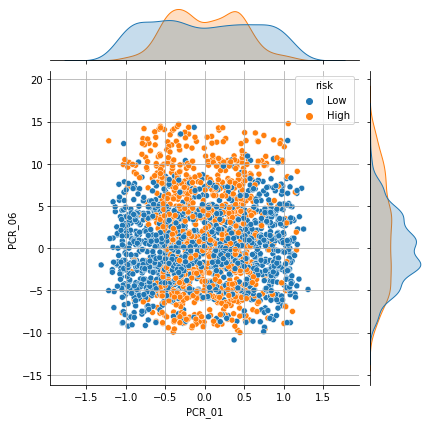
\includegraphics[scale=0.4]{q11_pcr_06_01_j_plot.png}
        \caption{Joint plot of PCR\_06 versus PCR\_01 with respect to risk}
        \label{fig:pcr_06_pcr_01_j_plot}
    \end{figure}
    \paragraph*{}
     Furthermore, from the scatter portion of the jointplot in figure \ref{fig:pcr_06_pcr_01_j_plot} we noticed a mostly separable form similar to the letter "H" where the "H" itself is made up of a high proportion of points with low risk surrounded by clusters of points of high risk. Therefore, we can conclude that in addition, \code{PCR\_06} will be important in predicting the \code{risk} class.
\subsection*{Q12:}
    \begin{figure}[H]
        \centering
        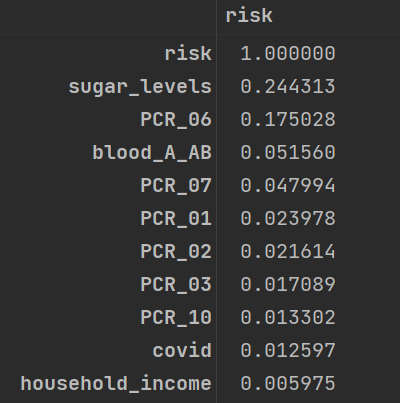
\includegraphics{images/q12.png}
        \caption{The 10 most correlated features to \code{risk}}
    \end{figure}
\section*{Part 3}
\subsection*{Q20:}
    \paragraph*{}
    In Q19, we used a 2 dimensional polynomial transform on the features within the primal objective of the SVM model. This approach is slower than the two dimensional kernel objective because it involves computing inner products between data points and the $w$ vector in high dimensions, whereas in the kernel case, the dual objective is used, which only involves computing the kernel function for 2 dimensional polynomials which is of much lower dimension (and finding and storing the $\alpha$s, which is not too computationally burdensome on the assumption that the support vectors are sparse).



\end{document}